\chapter{\sffamily Understanding the time evolution of probabilities}

{\bfseries\sffamily Concept.} To extend the formalism that we developed in the previous chapter to help us better understand the time evolution of state probabilities. With this knowledge we shall derive popular machine learning methods like Gaussian processes, as well as creating numerical procedures to directly solve for discrete state spaces. In the latter case these can be very intensive computations to perform, so in this chapter we shall also discuss the practical limitations of a fully numerical approach as well. For the mathematically-inclined, this chapter will take a detailed look at how our formalism can be extended to focus on the time evolution of probabilities. For the programmers, the software lives in this public Git repository: \href{https://github.com/umbralcalc/dennm-torch}{https://github.com/umbralcalc/dennm-torch}.

\section{\sffamily Probabilistic formalism}

In this section we will return to the stochadex formalism that we introduced in the first chapter of this book. As we discussed at that point; this formalism is appropriate for sampling from nearly every stochastic phenomenon that one can think of. We are going to extend this description to consider what happens to the probability that the state history matrix takes a particular set of values over time.

\begin{figure}[h]
\centering
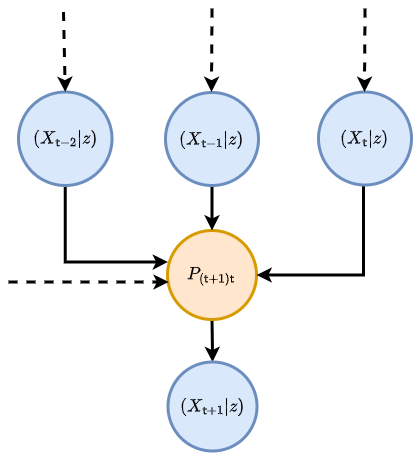
\includegraphics[width=8cm]{images/chapter-3-master-eq-graph.drawio.png}
\caption{Graph representation of Eqs.~(\ref{eq:master-x-cont}) and~(\ref{eq:master-x-cont-latest-row}).}
\label{fig:master-eqn}
\end{figure} 

So, how do we begin? In the first chapter, we defined the general stochastic process with the formula $X^{i}_{{\sf t}+1} = F^{i}_{{\sf t}+1}(X_{0:{\sf t}},z,{\sf t})$. This equation also has an implicit \emph{master equation} associated to it that fully describes the time evolution of the \emph{probability density function} $P_{{\sf t}+1}(X\vert z)$ of $X_{0:{\sf t}+1}=X$ given that the parameters of the process are $z$. This can be written as
%%
\begin{align}
P_{{\sf t}+1}(X\vert z) &= P_{{\sf t}}(X'\vert z) P_{({\sf t}+1){\sf t}}(x\vert X',z) \label{eq:master-x-cont}\,,
\end{align}
%%
where for the time being we are assuming the state space is continuous in each of the matrix elements and $P_{({\sf t}+1){\sf t}}(x\vert X',z)$ is the conditional probability that $X_{{\sf t}+1}=x$ given that $X_{0:{\sf t}}=X'$ at time ${\sf t}$ and the parameters of the process are $z$.

Consider what happens when we extend the chain of conditional probabilities in Eq.~(\ref{eq:master-x-cont}) back in time by one step. In doing so, we retrieve a joint probability of rows $X_{{\sf t}+1}=x$ and $X_{{\sf t}}=x'$ on the right hand side of the expression 
%%
\begin{align}
P_{{\sf t}+1}(X\vert z) &= P_{{\sf t}-1}(X''\vert z) P_{({\sf t}+1){\sf t}({\sf t}-1)}(x,x'\vert X'',z) \label{eq:master-x-pairwise-joint}\,.
\end{align}
%%
Since Eqs.~(\ref{eq:master-x-cont}) and~(\ref{eq:master-x-pairwise-joint}) are both valid ways to obtain $P_{{\sf t}+1}(X\vert z)$ we can average between them without loss of generality in the original expression, like this
%%
\begin{align}
P_{{\sf t}+1}(X\vert z) &= \frac{1}{2}\big[ P_{{\sf t}}(X'\vert z) P_{({\sf t}+1){\sf t}}(x\vert X',z) + P_{{\sf t}-1}(X''\vert z) P_{({\sf t}+1){\sf t}({\sf t}-1)}(x,x'\vert X'',z) \big]\,.
\end{align}
%%
Following this line of reasoning to its natural conclusion, Eq.~(\ref{eq:master-x-cont}) can hence be generalised to consider all possible joint distributions of rows at different timesteps like this
%%
\begin{align}
P_{{\sf t}+1}(X\vert z) &= \frac{1}{{\sf t}}\sum_{{\sf t}''=0}^{{\sf t}}P_{{\sf t}''}(X''\vert z) P_{({\sf t}+1){\sf t}\dots{\sf t}''}(x,x',\dots \vert X'',z) \label{eq:master-x-cont-sum-gen}\,.
\end{align}
%%

If we wanted to just look at the distribution over the latest row $X_{{\sf t}+1}=x$, we could achieve this through marginalisation over all of the previous matrix rows in Eq.~(\ref{eq:master-x-cont}) like this
%%
\begin{align}
P_{{\sf t}+1}(x\vert z) = \int_{\Omega_{{\sf t}}}{\rm d}X' P_{{\sf t}+1}(X\vert z) &= \int_{\Omega_{{\sf t}}}{\rm d}X' P_{{\sf t}}(X'\vert z) P_{({\sf t}+1){\sf t}}(x\vert X',z) \label{eq:master-x-cont-latest-row} \,.
\end{align}
%%
But what is $\Omega_{\sf t}$? You can think of this as just the domain of possible matrix $X'$ inputs into the integral which will depend on the specific stochastic process we are looking at. 

The symbol ${\rm d}X'$ in Eq.~(\ref{eq:master-x-cont-latest-row}) is our shorthand notation throughout the book for computing the sum of integrals over previous state history matrices which can further be reduced via Eq.~(\ref{eq:master-x-cont-sum-gen}) into a product of sub-domain integrals over each matrix row
%%
\begin{align}
P_{{\sf t}+1}(x\vert z) &= \frac{1}{{\sf t}}\sum_{{\sf t}''=0}^{{\sf t}} \bigg\lbrace \int_{\omega_{{\sf t}'}}{\rm d}^nx'...\int_{\Omega_{{\sf t}''}}{\rm d}X'' \bigg\rbrace \,P_{{\sf t}''}(X''\vert z) P_{({\sf t}+1){\sf t}\dots{\sf t}''}(x,x',... \vert X'',z) \\
&= \frac{1}{{\sf t}}\sum_{{\sf t}''=0}^{{\sf t}} \int_{\Omega_{{\sf t}''}}{\rm d}X'' P_{{\sf t}''}(X''\vert z) P_{({\sf t}+1){\sf t}''}(x \vert X'',z) \label{eq:master-x-cont-latest-row-gen} \,,
\end{align}
%%
where each row measure is a Cartesian product of $n$ elements (a Lebesgue measure), i.e.,
%%
\begin{align}
{\rm d}^nx = \prod_{i=0}^n{\rm d}x^i \,,
\end{align}
%%
and lowercase $x, x', \dots$ values will always refer to individual rows within the state matrices. Note that $1/{\sf t}$ here is a normalisation factor --- this just normalises the sum of all probabilities to 1 given that there is a sum over ${\sf t}'$. Note also that, if the process is defined over continuous time, we would need to replace 
%%
\begin{align}
\frac{1}{{\sf t}}\sum_{{\sf t}'=0}^{{\sf t}} \rightarrow \frac{1}{t({\sf t})}\sum_{{\sf t}'=0}^{{\sf t}}\delta t({\sf t}') \,.
\end{align}
%%

To try and understand what Eqs.~(\ref{eq:master-x-cont}) and~(\ref{eq:master-x-cont-latest-row}) are saying, we find it's helpful to think of an iterative relationship between probabilities; each of which is connected by their relative conditional probabilities. This kind of thinking is also illustrated in Fig.~\ref{fig:master-eqn}.

Before we move onto the learning algorithm and software design sections, let's take a quick mathematical look at some important sub-categories of stochastic process which exist within the general description provided by Eqs.~(\ref{eq:master-x-cont}) and~(\ref{eq:master-x-cont-latest-row}). For Markovian phenomena, the equations no longer depend on timesteps older than the immediately previous one, hence Eq.~(\ref{eq:master-x-cont-latest-row}) reduces to just
%%
\begin{align}
P_{{\sf t}+1}(x\vert z) &= \int_{\omega_{\sf t}}{\rm d}^nx' \, P_{\sf t}(x'\vert z) P_{({\sf t}+1){\sf t}}(x\vert x',z) \label{eq:master-x-cont-markov} \,.
\end{align}
%%
By performing a Kramers-Moyal expansion on the $P_{({\sf t}+1){\sf t}}(x\vert x',z)$ distribution up to second order,\footnote{The Pawula theorem~\cite{pawula1967generalizations} states that this is, in fact, as far as we can truncate up to unless we include an infinite number of expansion terms.} we can approximate the right hand side of Eq.~(\ref{eq:master-x-cont-markov}) like this 
%%
\begin{align}
P_{({\sf t}+1)}(x\vert z) &\simeq P_{{\sf t}}(x\vert z) - \sum_{i=0}^n\frac{\partial}{\partial x^i}\bigg[ f_{{\sf t}}(x,z)P_{{\sf t}}(x\vert z)\bigg] + \frac{1}{2}\sum_{i=0}^n\sum_{j=0}^n\frac{\partial}{\partial x^i}\frac{\partial}{\partial x^j}\bigg[ K_{{\sf t}}(x,z)P_{{\sf t}}(x\vert z)\bigg] \label{eq:kramers-moyal} \,,
\end{align}
%%
where the components of $f_{{\sf t}}(x,z)$ and $K_{{\sf t}}(x,z)$ have been defined as
%%
\begin{align}
f^i_{{\sf t}}(x,z) &= \int_{\omega_{{\sf t}+1}} {\rm d}^nx' (x'-x)^iP_{({\sf t}+1){\sf t}}(x'\vert x,z) \\
K^{ij}_{{\sf t}}(x,z) &= \int_{\omega_{{\sf t}+1}} {\rm d}^nx' (x'-x)^i(x'-x)^jP_{({\sf t}+1){\sf t}}(x'\vert x,z)\,.
\end{align}
%%

By inspection of Eq.~(\ref{eq:kramers-moyal}) we can define the `probability current'
%%
\begin{align}
J_{{\sf t}}(x,z) &= f_{{\sf t}}(x,z)P_{{\sf t}}(x\vert z) - \frac{1}{2}\sum_{j=0}^{n}\frac{\partial}{\partial x^j}\bigg[ K_{{\sf t}}(x,z)P_{{\sf t}}(x\vert z)\bigg] \,.
\end{align}
%%
If the probability current vanishes $J_{{\sf t}}(x,z)=0$ individually (this also implies that the distribution is stationary such that $P_{{\sf t}+1}(x\vert z)=P_{{\sf t}}(x\vert z)$), the implicit solution of Eq.~(\ref{eq:kramers-moyal}) can be found to be
%%
\begin{align}
P_{{\sf t}}(x\vert z) \propto K_{{\sf t}}^{-1}(x,z)\exp \bigg[ \int {\rm d}^nx\, K^{-1}_{{\sf t}}(x,z)f_{{\sf t}}(x,z)\bigg] \,.
\end{align}
%%

An analog of Eq.~(\ref{eq:master-x-cont-latest-row}) exists for discrete state spaces as well. We just need to replace the integral with a sum and the schematic would look something like this
%%
\begin{align}
P_{{\sf t}+1}(x\vert z) &= \sum_{\Omega_{{\sf t}}} P_{{\sf t}}(X'\vert z) P_{({\sf t}+1){\sf t}}(x \vert X', z) \label{eq:master-x-disc} \,,
\end{align}
%%
where we note that the $P$'s in the expression above all now refer to \emph{probability mass functions}.

\section{\sffamily Learning algorithms}

We can approximate the probability $P_{{\sf t}+1}(X\vert z)$ with a logarithmic expansion like this
%%
\begin{align}
\ln P_{{\sf t}+1}(X\vert z) &\simeq \ln P_{{\sf t}+1}(X_*\vert z) + \frac{1}{2}\sum_{{\sf t}'=0}^{{\sf t}+1}\sum_{i=0}^{n}\sum_{j=0}^{n} (x-x_*)^i {\cal I}^{ij}_{({\sf t}+1){\sf t}'}(x_*,x'_*) (x'-x'_*)^j \label{eq:second-order-log-expansion} \\
{\cal I}^{ij}_{({\sf t}+1){\sf t}'}(x_*,x'_*) &= \frac{\partial}{\partial x^i}\frac{\partial}{\partial (x')^j}\ln P_{{\sf t}+1}(X\vert z) \bigg\vert_{X=X_*} \,,
\end{align}
%% 
where the values for $X=X_*$ are defined by the vanishing of the first derivative, i.e., these are chosen such that
%%
\begin{align}
\frac{\partial}{\partial x^i}\ln P_{{\sf t}+1}(X\vert z) \bigg\vert_{X=X_*} &= 0 \,.
\end{align}
%%
If we keep the truncation up to second order in Eq.~(\ref{eq:second-order-log-expansion}), note that this expression implies a pairwise correlation structure of the form
%%
\begin{align}
P_{{\sf t}+1}(X\vert z) &\rightarrow \prod_{{\sf t}'=0}^{{\sf t}}P_{({\sf t}+1){\sf t}'}(x,x'\vert z) = \prod_{{\sf t}'=0}^{{\sf t}}P_{{\sf t}'}(x'\vert z)P_{({\sf t}+1){\sf t}'}(x\vert x', z) \,.
\end{align}
%%
Given this pairwise temporal correlation structure, Eq.~(\ref{eq:master-x-cont-latest-row-gen}) reduces to this simpler sum of integrals
%%
\begin{align}
P_{{\sf t}+1}(x\vert z) &= \frac{1}{{\sf t}}\sum_{{\sf t}'=0}^{{\sf t}}\int_{\omega_{{\sf t}'}}{\rm d}^nx' P_{{\sf t}'}(x'\vert z)P_{({\sf t}+1){\sf t}'}(x\vert x',z) \label{eq:second-order-correl} \,.
\end{align}
%%

In a similar fashion, we can increase the expansion order of Eq.~(\ref{eq:second-order-log-expansion}) to include third-order correlations such that 
%%
\begin{align}
P_{{\sf t}+1}(X\vert z) &\rightarrow \prod_{{\sf t}'=0}^{{\sf t}}\prod_{{\sf t}''=0}^{{\sf t}'-1} P_{{\sf t}'{\sf t}''}(x',x''\vert z)P_{({\sf t}+1){\sf t}'{\sf t}''}(x\vert x',x'',z) \,,
\end{align}
%%
and, in this instance, one can show that Eq.~(\ref{eq:master-x-cont-latest-row-gen}) reduces to
%%
\begin{align}
P_{{\sf t}+1}(x\vert z) &= \frac{1}{{\sf t}}\sum_{{\sf t}'=0}^{{\sf t}}\frac{1}{{\sf t}'-1}\sum_{{\sf t}''=0}^{{\sf t}'-1}\int_{\omega_{{\sf t}'}}{\rm d}^nx'\int_{\omega_{{\sf t}''}}{\rm d}^nx'' P_{{\sf t}'{\sf t}''}(x',x''\vert z)P_{({\sf t}+1){\sf t}'{\sf t}''}(x\vert x',x'',z) \label{eq:third-order-correl} \,.
\end{align}
%%
Using $P_{{\sf t}'{\sf t}''}(x',x''\vert z) = P_{{\sf t}''}(x''\vert z) P_{{\sf t}'{\sf t}''}(x'\vert x'', z)$ one can also show that this integral is a marginalisation of this expression
%%
\begin{align}
P_{({\sf t}+1){\sf t}''}(x\vert x'', z) &= \frac{1}{{\sf t}}\sum_{{\sf t}'=0}^{{\sf t}}\int_{\omega_{{\sf t}'}}{\rm d}^nx'P_{{\sf t}'{\sf t}''}(x'\vert x'',z)P_{({\sf t}+1){\sf t}'{\sf t}''}(x\vert x',x'',z) \,,
\end{align}
%%
which describes the time evolution of the conditional probabilities.

Let's imagine that $x$ is just a scalar (as opposed to a row vector) for simplicity in the expressions. We can then discretise the 1D space over $x$ into separate $i$-labelled regions such that $[P]^i_{{\sf t}+1} - [P]^i_{{\sf t}} = {\cal J}^i_{{\sf t}+1}$, where the probability current ${\cal J}^i_{{\sf t}+1}$ for the factorised processes above would be defined as
%%
\begin{align}
{\cal J}^i_{{\sf t}+1} &= - [P]^i_{{\sf t}} + \frac{1}{{\sf t}}\sum^{{\sf t}}_{{\sf t}'=0}\sum_{i'=0}^N\Delta x[P]^{i'}_{{\sf t}'}[P]^{ii'}_{({\sf t}+1){\sf t}'} \\
{\cal J}^i_{{\sf t}+1} &= - [P]^i_{{\sf t}} + \frac{1}{{\sf t}}\sum^{{\sf t}}_{{\sf t}'=1}\frac{1}{{\sf t}'-1}\sum^{{\sf t}'-1}_{{\sf t}''=0}\sum_{i'=0}^N\sum_{i''=0}^N\Delta x^2[P]^{i''}_{{\sf t}''}[P]^{i'i''}_{{\sf t}'{\sf t}''}[P]^{ii'i''}_{({\sf t}+1){\sf t}'{\sf t}''}\,.
\end{align}
%%

The $[P]^{ii'i''}_{({\sf t}+1){\sf t}'{\sf t}''}$ tensor, in particular, will have $N^3{\sf t}({\sf t}^2-1)$ elements. Note that the third-order temporal correlations can be evolved by identifying the pairwise conditional probabilities as time-dependent state variables and evolving them according to the following relation
%%
\begin{align}
[P]^{ii''}_{({\sf t}+1){\sf t}''} &= \frac{1}{{\sf t}}\sum^{{\sf t}}_{{\sf t}'=1}\sum_{i'=0}^N\Delta x[P]^{i'i''}_{{\sf t}'{\sf t}''}[P]^{ii'i''}_{({\sf t}+1){\sf t}'{\sf t}''}\,.
\end{align}
%%

\textcolor{red}{
\begin{itemize}
\item{Main point of this section is for Gaussian (and higher-order) learning processes + the adjoint master equation learning method before this point}
\item{Add some diagrams for the higher-order correlation expressions.}
\item{Also add note that we explored the direct numerical evaluation of the higher-order process in this repository: \href{https://github.com/umbralcalc/dennm-torch}{https://github.com/umbralcalc/dennm-torch}.}
\end{itemize}
}

\section{\sffamily Software design}

\textcolor{red}{
\begin{itemize}
\item{Add a software design section and some examples} 
\item{Dev the learnadex with Gotch to achieve all this stuff}
\end{itemize}
}

    